\clearpage
\newpage

\chapter{Questions and Answers}
\label{ch-QA}


\paragraph{Correction: Fixed boundary condition outside the damping layers} ~

Before the QA, in Day-2, there was a modeling error where the boundary of the damping layers was not fixed.
This boundary condition has been corrected in the Real-ESSI-Day3 image. 
The correct boundary condition should be perpendicular to the wall, as shown in Fig.\ref{fig_BC_xy}.

\begin{figure}[H]
  \centering
  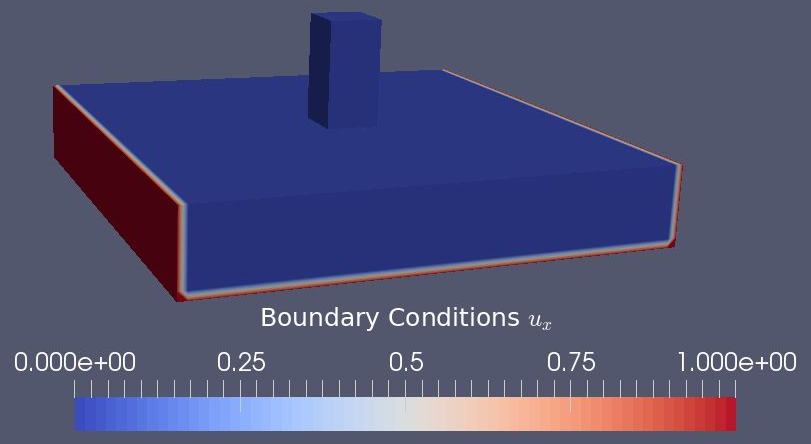
\includegraphics[width = 7.4cm]{./Figure-files/QA/boundary_condition_ux.png}
  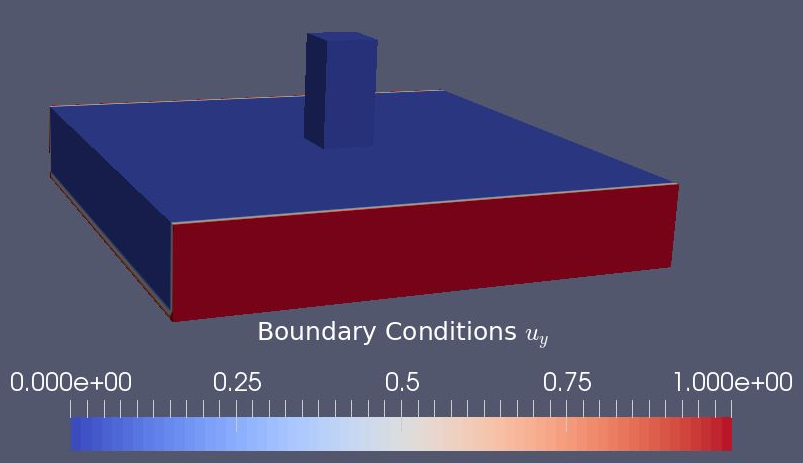
\includegraphics[width = 7cm]{./Figure-files/QA/boundary_condition_uy.png}
  \caption{Boundary Condition at $x$ and $y$ direction respectively.}
  \label{fig_BC_xy}
\end{figure}

After the correction, the results is shown in Fig.\ref{fig_BC_xy_ans}.
\begin{figure}[H]
  \centering
  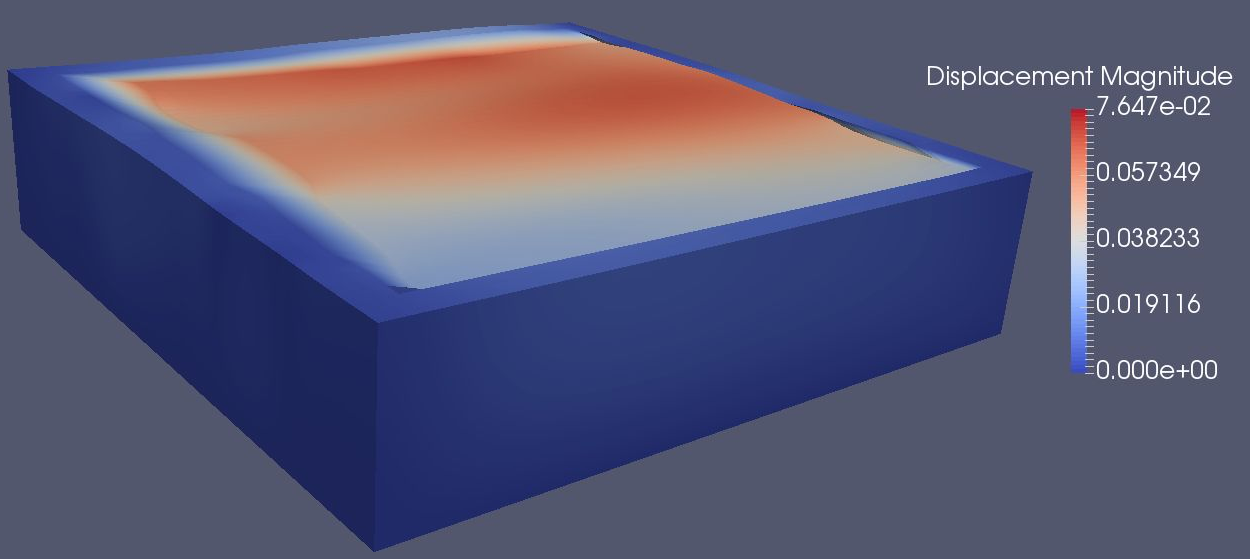
\includegraphics[width = 7cm]{./Figure-files/QA/DRM_SW4_motion.png}
  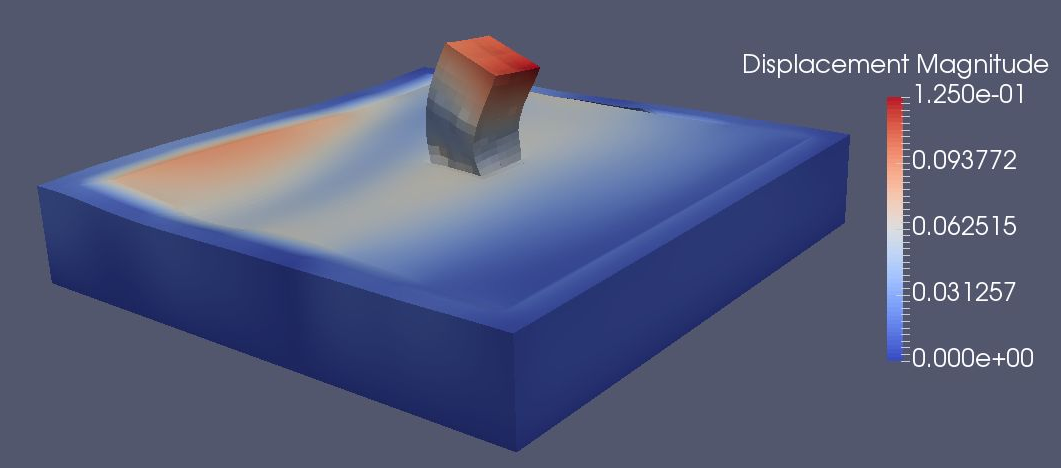
\includegraphics[width = 7cm]{./Figure-files/QA/shell_structure_correction.png}
  \caption{Illustrative Results with the correct boundary condition}
  \label{fig_BC_xy_ans}
\end{figure}
You can also reproduce this result on your instance by yourself.




% ==========================================================
% ==========================================================
% ==========================================================
% ==========================================================
\clearpage
\newpage

\paragraph{Question: The 3D soil-structure model is fancy. However, we want to see how to build a very simple model from scratch. } ~

\textbf{Answer:} The short-courses focus on the capability of Real-ESSI. In Day 3, some basic example may be illustrated step by step if we have time. For example, we can do a simple cantilever.

Reminder: there are also other preprocessing converters like SASSI2ESSI.
By the way, you are welcome to develop other converters, like NASTRAN to ESSI.


\paragraph{Question: Will the specified external load accumulates or replaces the existing load if I add the load to 1 DOF twice?} ~

\textbf{Answer:} 
The load will accumulate if you define the load correctly.
Every load has the unique load tag, you can add two different load tags on the same node twice. The simulation goes over all the load tags and adds them up. 

On the other side, if you define with the same load-tag, you will get a warning which reminds you that the load-tag has already been used.



\paragraph{Question: Could I download the examples/results to my local computer?} ~

\textbf{Answer:} 
On MacBook/Linux, you can always use command $scp/rsync$ to download/upload examples/results between your AWS instances and your local computers.
In Windows, you can install Putty to use $scp/rsync$.
Additionally, starting from Image Real-ESSI-Day-3, you can host your own website automatically to download result from AWS to your local computer by the following steps:
\begin{enumerate}
	\item When you launch your instances, in the Security Group, add a new HTTP rule for your website, as shown in~\ref{fig_Security_group_AWS}.
	\item Copy the files (you want to download) to the folder $/home/ubuntu/website/html/public/$.
(Note that the data inside this folder is public and any can see and download it.)
\end{enumerate}

Then you can download these files through this website:
$your-Public-DNS/public/$.

By the way, you can always pass the data through your own email.

\begin{figure}[H]
  \centering
  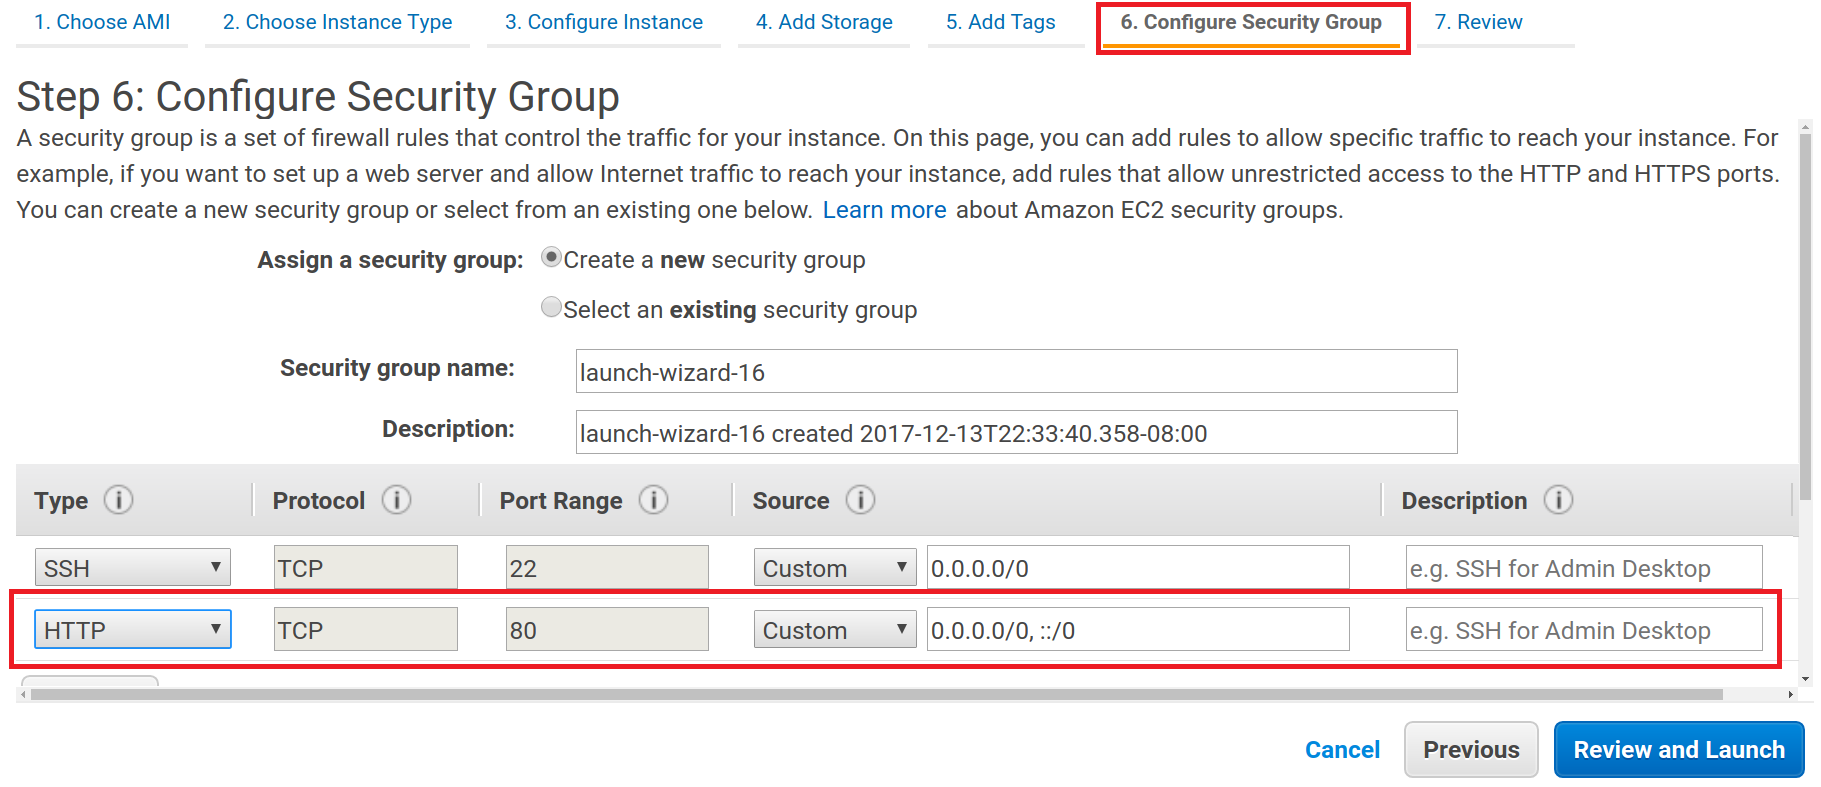
\includegraphics[width = 15cm]{./Figure-files/QA/security_group.png}
  \caption{Specify Security Group for Download Results from AWS}
  \label{fig_Security_group_AWS}
\end{figure}




\paragraph{Question: Nonlinear analysis is always slow, could I have the results ready for view?} ~

\textbf{Answer:} 
Sure, in Day-3, there will be two Real-ESSI-images.
\begin{itemize}
	\item Real-ESSI-Day3 with 30GB (Real-ESSI Input only).
	\item Real-ESSI-ans with 100GB (Real-ESSI Input and Output).
\end{itemize}



\paragraph{Question: The AWS EC2 instance is only 30GB. What if I run out of disk space?} ~

\textbf{Answer:} 
You can attach new disk (Volumes) to your instance during runtime. You can also add more disk space before you launch the instance, as shown in Fig.~\ref{fig_Security_group_AWS}.

\begin{figure}[H]
  \centering
  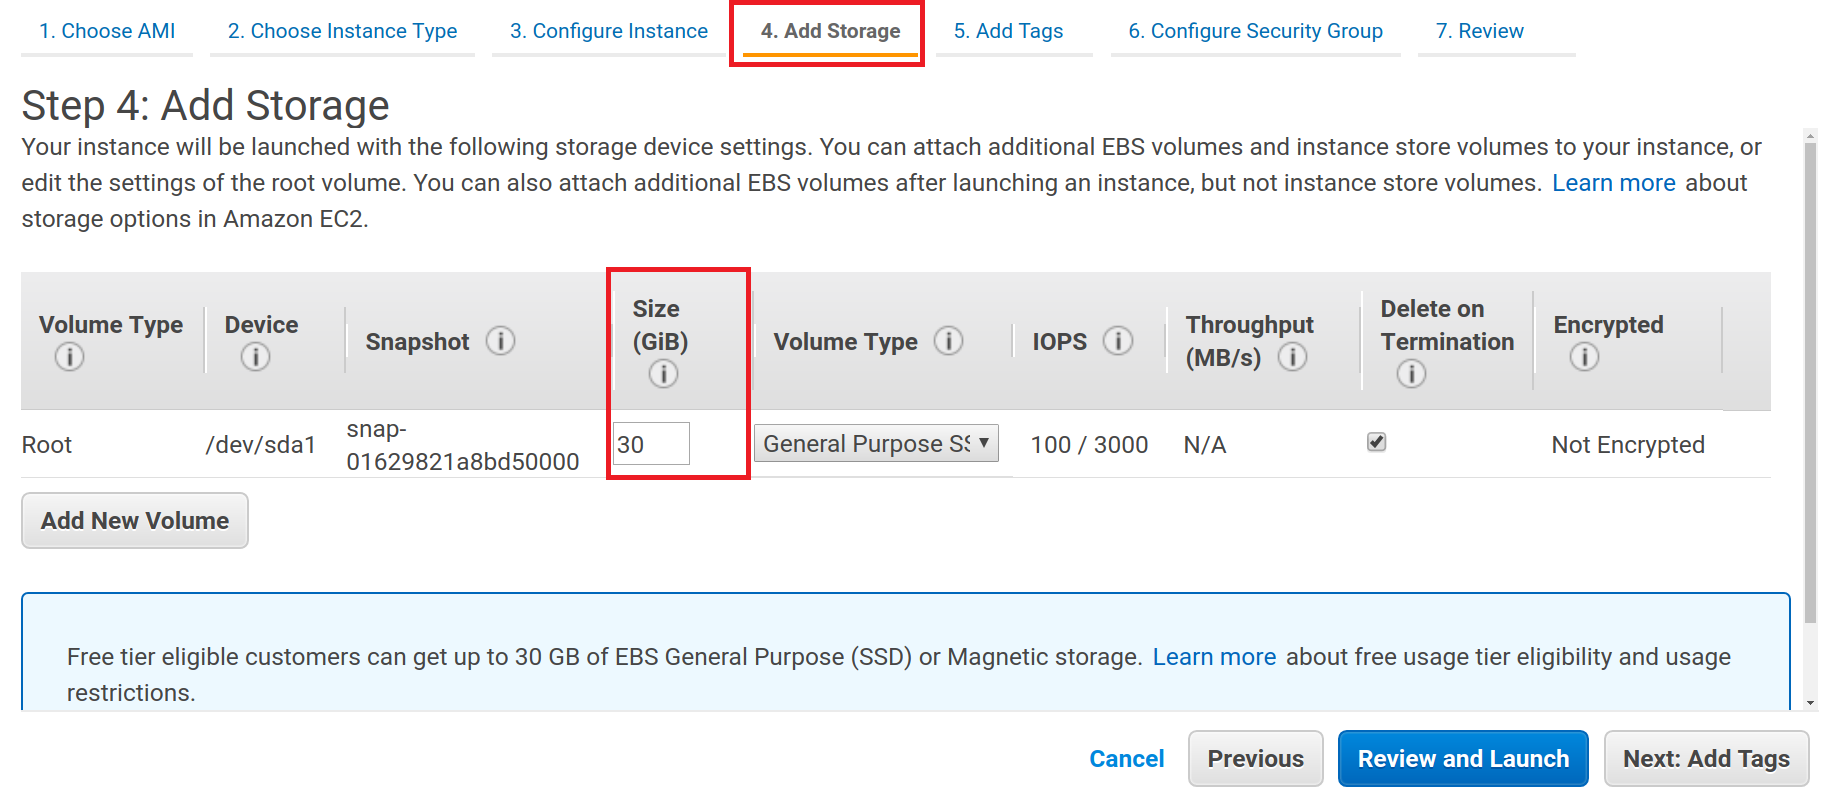
\includegraphics[width = 15cm]{./Figure-files/QA/specify_storage_time.png}
  \caption{Specify Storage Volume for Huge Models.}
  \label{fig_Specify_storage_model}
\end{figure}




\paragraph{Question: Why do we use the instance type c4.2xlarge?} ~

\textbf{Answer:} 
Actually, you can launch any Real-ESSI-Image on any instance. The Image is like a CD, you can play a CD on any player.
However, there is a price issue. The instance price is a combination of the CPU type, Memory Space (RAM), the network, etc. For our type of problem, we focus on the compute speed, so we choose the C-instances (Compute-Optimized Instances), which is a good combination of CPU, RAM, and Network. In addition, on c4.2 instances, most examples can be finished within 30 minutes, which is a good practice for the short-course. 


\paragraph{Question: Why I can only see a part of the output?} ~

\textbf{Answer:} 
Parallel Real-ESSI are outputing the results in multiple files, the output of the master process is named "h5.output", while the output of slave processes are named "h5.XX.output". You need to open the output through the master output file.
All of partitions is shown in Fig.~\ref{fig_Specify_storage_model}.
\begin{figure}[H]
  \centering
  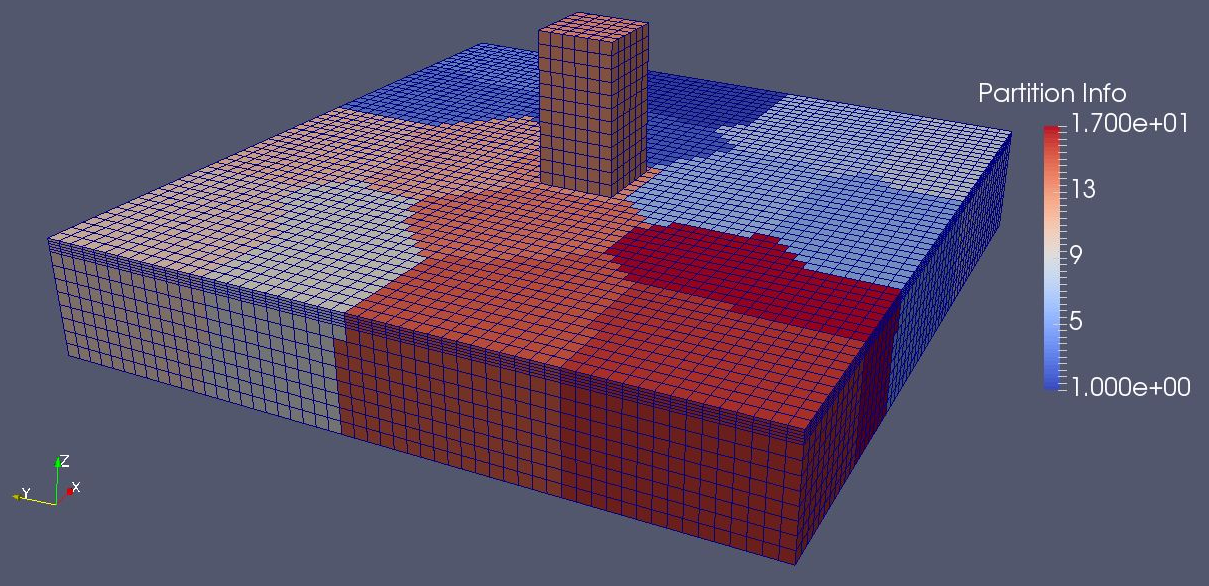
\includegraphics[width = 10cm]{./Figure-files/QA/Partition_info.png}
  \caption{Open the Master Output Files to View All the Results}
  \label{fig_Specify_storage_model}
\end{figure}




\paragraph{Question: In my earthquake simulation, I never try any time step greater than 0.005 second? Why are you using such a big time step? (e.g. 0.04 second)} ~

\textbf{Answer:} 
The short-course wants everyone to complete the Real-ESSI simulation during the class. So we use short-duration earthquake with big time-steps on purpose to illustrate the structural behavior under earthquake. Real-ESSI has the full capability to run the simulation with very small time step.


\paragraph{Question: Could I still use the Real-ESSI-Image when I go back to my country?} ~

\textbf{Answer:} 
Absolutely. Real-ESSI-Image can be accessed in other country as well. We once tested the availability with our colleague through Italy. Please ask Prof.Jeremi{\'c} for more details about the availability of Real-ESSI-Image.


\paragraph{Reminder} ~

Last but not least, remember to terminate your instances after the short-course. 
During this short-course, when you are using AWS, you only pay to Amazon. (The Real-ESSI-Image you are using are free for the moment.)
Your bill of AWS will come monthly, just like your electricity bill from PG\&E.






